\documentclass[a4paper]{article}
\usepackage[utf8]{inputenc}
\usepackage[T1]{fontenc}
\usepackage{graphicx}
\usepackage{longtable}
\usepackage{hyperref}
\usepackage{caption}

\usepackage[margin=1.5in]{geometry}
\usepackage{setspace}
\onehalfspacing

\usepackage{fancyhdr}
\pagestyle{fancy}
\fancyhead{}
\fancyfoot{}
\fancyhead[LE,RO]{\leftmark}
\fancyhead[RE,LO]{Harry Potter}
\fancyfoot[C]{\thepage}
\renewcommand{\headrulewidth}{0.4pt}
\renewcommand{\footrulewidth}{0pt}

\usepackage[backend=biber, style=numeric]{biblatex}
\addbibresource{./references.bib}

\usepackage[numbib,notlof,notlot,nottoc]{tocbibind}
\pagenumbering{gobble}

\begin{document}
	
\begin{titlepage}

    \newcommand{\HRule}{\rule{\linewidth}{0.1mm}} % Defines a new command for the horizontal lines, change thickness here

    \center % Center everything on the page
	
   \textsc{\Large Master Thesis}\\[0.5cm] % Major heading such as course name
	    
    %----------------------------------------------------------------------------------------
    %	TITLE SECTION
    %----------------------------------------------------------------------------------------
    
    \HRule \\[0.4cm]
    { \huge \bfseries How to perform an Expecto Patronum }\\[0.7cm] % Title of your document
    \HRule \\[0.4cm]
    
    \vspace{2cm}

    %----------------------------------------------------------------------------------------
    %	INSTITUTION SECTION
    %----------------------------------------------------------------------------------------
    
    % LOGO 
    
\includegraphics[width=0.15\textwidth]{img/hogwarts.png}\\[1cm] % Include a department/university logo - this will require the graphicx package
    
   \textsc{\LARGE Hogwarts, School of Witchcraft and Wizardry}\\[0.5cm] % Name of your university/college
   
   % DEPARTMENT
    \large
    Department of Defence against the Dark Arts \\
    Faculty of Art of Magic \\
   
	\vspace{3cm}
	
    %----------------------------------------------------------------------------------------
    %	AUTHOR SECTION
    %----------------------------------------------------------------------------------------
    
	\large
	\textbf{Author}: Harry Potter\\
	\large
	\textbf{Supervisor}: Severus Snape
	
	\vspace{2cm}

    %----------------------------------------------------------------------------------------
    %	DATE SECTION
    %----------------------------------------------------------------------------------------

    {\large \today}\\[1cm] % Date, change the \today to a set date if you want to be precise

    \vfill  % Fill the rest of the page with whitespace
    

\end{titlepage}


\pagenumbering{Roman}
\tableofcontents
\clearpage
\listoffigures
\clearpage
\listoftables
\clearpage

\pagenumbering{arabic}

\section{Section One}
\label{sec:section_one}
\begin{figure}[htbp]
    \centering
    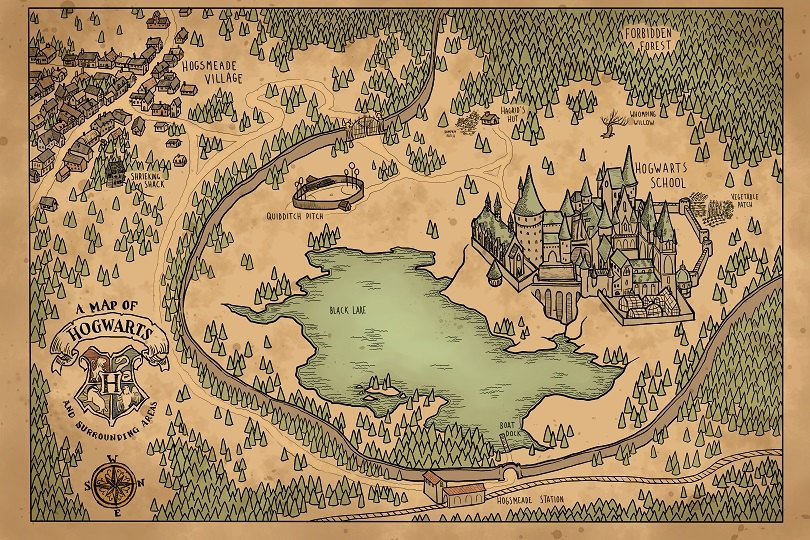
\includegraphics[width=.9\linewidth]{./figures/hogwarts_map.jpg}
    \caption{Map of Hogwarts}
    \label{figure:hogwarts_map}
\end{figure}
See Figure \ref{figure:hogwarts_map} for details. Additional information can be
found in the footnote\footnote{Image taken from \url{https://www.jstor.org/stable/25148625}.}. \\

This is a example sentence for citation \cite{hevner04_desig_scien_infor_system_resear}


\clearpage

\section{Section Two}
\label{sec:section_two}
\begin{longtable}{l|ccccc}
  \caption{Sample Table}
  \label{table:table-1}
  \\
  \hline
  \hline
  Id & Col 1 & Col 2 & Col 3 & Col 4 & Col 5\\
  \hline
  1 & Col 1 & Col 2 & Col 3 & Col 4 & Col 5\\
  2 & Col 1 & Col 2 & Col 3 & Col 4 & Col 5\\
  3 & Col 1 & Col 2 & Col 3 & Col 4 & Col 5\\
  4 & Col 1 & Col 2 & Col 3 & Col 4 & Col 5\\
  5 & Col 1 & Col 2 & Col 3 & Col 4 & Col 5\\
  \hline
  \hline
\end{longtable}
\clearpage

\printbibliography

\end{document}
